\documentclass[11pt,a4paper]{article}
\usepackage[utf8]{inputenc}
\usepackage[italian]{babel}
\usepackage{amsmath}
\usepackage{amsfonts}
\usepackage{amssymb}
\usepackage{array}
\usepackage{graphicx}
\usepackage{multirow}
\usepackage{color,colortbl}
\usepackage[hidelinks]{hyperref}
\usepackage{fancyhdr}
\usepackage{tabularx}
\usepackage[left=2cm,right=2cm,top=2cm,bottom=3cm]{geometry}
\usepackage{enumerate}
\usepackage{lastpage}
\usepackage{hyperref}
\hypersetup{colorlinks,urlcolor=blue,linkcolor=black}

\pagestyle{fancy}
\fancyhf{}
\lhead{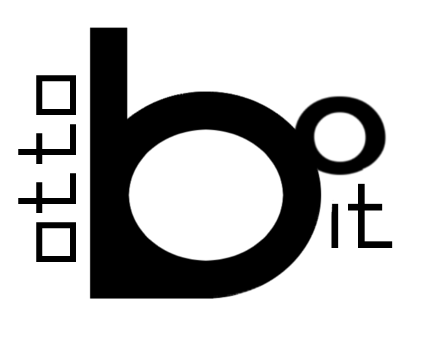
\includegraphics[scale=0.07]{images/logo.png}}

\renewcommand {\footrulewidth}{0.2mm}
\lfoot {Norme di progetto}
\rfoot{Pagina \thepage\ di \pageref{LastPage}}

\definecolor{LightBlue}{rgb}{0,0,0.5}
\definecolor{Gray}{gray}{0.8}
\definecolor{LightGray}{gray}{0.9}




\usepackage{lipsum}
\usepackage{verbatim}



\setcounter{tocdepth}{4}
\setcounter{secnumdepth}{4}



\begin{document}
	\begin{titlepage}
  \centering
	\scshape
	
	\vspace*{2cm}
	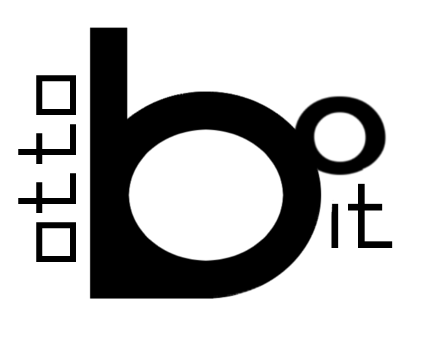
\includegraphics[scale=0.7]{images/logo.png}
	\rule{\linewidth}{0.2mm}\\[0.37cm]
	{\Huge Piano di progetto}\\
	\rule{\linewidth}{0.2mm}\\[1cm]
	{\LARGE\bfseries Progetto Colletta - Gruppo OttoBit}\\[1cm]
	
	
	
	\begin{tabular}{>{\columncolor{Gray}}r | >{\normalfont}l}
		\rowcolor{LightBlue}		
		\multicolumn{2}{c}{\color{white}{Informazioni sul documento}}\\
		Versione & 1.0.0 \\
		Redazione & Benedetto Cosentino\\
							& Enrico Marcato\\
 		Verifica & Giovanni Peron\\
 		Responsabile & Benedetto Cosentino\\
 		Uso & Esterno\\
 																 		& Prof. Tullio Vardanega\\
 																		& Prof. Riccardo Cardin\\
 		\multirow[t]{-3}{*}{Destinatari}	& MIVOQ s.r.l\\
 		\hline
	\end{tabular}
\end{titlepage}

	
	\newpage
	\section*{\centering Registro delle modifiche}
	\begin{tabularx}{\textwidth}{ c | c | X | c | X }
		\rowcolor{LightBlue}
		\color{white}\bfseries Versione & \color{white}\bfseries Data & \multicolumn{1}{c}{\color{white}\bfseries Autore}
		 & \color{white}\bfseries Ruolo & \multicolumn{1}{c}{\color{white}\bfseries Descrizione}\\[0.25cm]
		 1.0.0 & 2019-01-11 & Benedetto Cosentino & Responsabile & Approvazione documento \\ \hline
		 0.2.0 & 2018-12-27 & Michele Bortone & Verificatore & Verifica documento \\ \hline
		0.1.2 & 2018-12-20 & Giovanni Bergo \newline Gianmarco Pettenuzzo & Amministratore & Aggiornamento Norme di progetto \\ \hline
		0.1.1 & 2018-12-20 & Eleonora Peagno & Amministratore & Aggiornamento processi primari \\ \hline
		0.1.0 & 2018-12-18 & Michele Bortone & Verificatore & Verifica documento \\ \hline
		0.0.6 & 2018-12-15 & Enrico Marcato & Amministratore & Stesura processi di \newline sviluppo \\ \hline
		0.0.5 & 2018-12-14 & Eleonora Peagno & Amministratore & Stesura processi primari \\ \hline
		0.0.4 & 2018-12-11 & Eleonora Peagno & Amministratore & Introduzione \\ \hline
	0.0.3 & 2018-12-16 & Giovanni Bergo \newline Gianmarco Pettenuzzo & Amministratore & Aggiornamento Norme di progetto \\ \hline
	0.0.2 & 2018-12-14 & Giovanni Bergo \newline Gianmarco Pettenuzzo & Amministratore & Stesura processi \newline organizzativi \\ \hline
	0.0.1 & 2018-12-11 & Giovanni Bergo \newline Gianmarco Pettenuzzo & Amministratore & Stesura processi di \newline supporto \\ \hline


	
		
	
	\end{tabularx}

	\newpage	

	\renewcommand  \contentsname {\Large Indice} 
	
	\tableofcontents
	\newpage
	
	\section{Introduzione}
	\subsection{Scopo del documento}
	Lo scopo delle \textit{Norme di progetto} è formalizzare uno standard per la stesura dei documenti durante tutto il percorso del progetto$^*$ didattico. Inoltre, si vuole normare il processo di sviluppo delle attività svolte al suo interno. 
	\\Ogni componente del gruppo è tenuto a farne riferimento così da poter ottenere dei documenti omogenei tra loro e, di conseguenza, più facili da verificare. 
	Tutte le regole qui descritte sono state elaborate dall'intero gruppo, il quale deve approvare eventuali modifiche, aggiunte o rimozioni.
	\subsection{Scopo del prodotto}
	Lo scopo del prodotto è creare una piattaforma collaborativa di raccolta dati su cui sia possibile predisporre e/o svolgere esercizi di analisi grammaticale. La raccolta vorrebbe avere il fine di fornire a sviluppatori e ricercatori dati sufficienti per applicare metodi di apprendimento automatico$^*$. Nello specifico si vorrebbe poter insegnare ad un elaboratore a svolgere gli stessi esercizi proposti agli utenti, divenendo una sorta di correttore automatico.  
	Le componenti principali del prodotto saranno quindi:
	\begin{itemize}
		\item un'interfaccia web, su cui verranno predisposti e svolti gli esercizi;
		\item un servizio esistente di database$^*$;
		\item il servizio esistente open-source per il pos-tagging.
	\end{itemize}
	
	\subsection{Riferimenti}
	Segue l'elenco dei riferimenti utilizzati dal gruppo:
	\subsubsection{Riferimenti normativi}
	\begin{itemize}
		\item ISO/IEC 12207$^*$
		\footnote{\url {https://it.wikipedia.org/wiki/ISO\_12207}}
		
		\item ISO/IEC 15504$^*$
		\footnote{\url {https://en.wikipedia.org/wiki/ISO/IEC\_15504}}
		\item ISO/IEC 9126$^*$
		\footnote{\url {https://it.wikipedia.org/wiki/ISO/IEC\_9126}}
	\end{itemize}	
	
	\subsubsection{Riferimenti informativi}
	\begin{itemize}
		\item Slide del corso "Ingegneria del software" - Processi di sviluppo 
		\footnote{\url{https://www.math.unipd.it/~tullio/IS-1/2018/Dispense/L03.pdf}}
		\item Slide del corso "Ingegneria del software" - Ciclo di vita 
		\footnote{\url{https://www.math.unipd.it/~tullio/IS-1/2018/Dispense/L05.pdf}}
		\item Capitolato 2
		\footnote{\url{https://www.math.unipd.it/~tullio/IS-1/2018/Progetto/C2.pdf}}
		\item Wikipedia/GitLab
		\footnote{\url {https://it.wikipedia.org/wiki/GitLab}}
	\end{itemize}					
	\newpage
	
	\section{Processi primari}
	\subsection{Ricerca sulle tecnologie} 
	Questa fase consiste nella ricerca di informazioni su software, librerie e tutte le tecnologie che sono state ritenute utili per una o più fasi di sviluppo del progetto. Le tecnologie analizzate  sono quelle suggerite dalla proponente e quelle ritenute utili sulla base delle esperienze personali dei membri del gruppo. 
	
	
	\subsection{Normazione}
	Uno dei compiti dell'Amministratore di progetto, è quello di stilare la lista delle regole che tutti i componenti del gruppo dovranno seguire nella stesura dei documenti e nello svolgimento delle attività assegnate a ciascuno. Con l'avanzamento dello sviluppo del progetto, tali regole potrebbero subire delle variazioni e/o delle aggiunte poiché, durante lo sviluppo stesso, si potranno acquisire nuove conoscenze o incontrare difficoltà tali da portare alla rielaborazione delle succitate regole. Si potrebbe anche decidere di utilizzare uno strumento diverso da quelli preventivati e, anche per questo, andranno stabilite regole specifiche.\\
	\textbf{Prodotto dell'attività}: \textit{Norme di progetto}
	
	\subsection{Studio di fattibilità}
	Nella prima fase dello sviluppo del progetto, agli Analisti è richiesto di approfondire i requisiti di ogni capitolato proposto dai committenti così da capirne l'entità e decidere se accettare o meno il contratto. Nello specifico, per ogni capitolato si vuole conoscere:
	\begin{itemize}
		\item il contesto di utilizzo e lo scopo del prodotto da realizzare;
		\item le tecnologie di cui è richiesto l'utilizzo per lo svolgimento del progetto;
		\item l'interesse ed il gradimento del gruppo verso l'obiettivo finale del capitolato.
	\end{itemize}
	\textbf{Prodotto dell'attività}: \textit{Studio di fattibilità}
	
	\subsection{Analisi dei requisiti}
	Gli Analisti dovranno definire l'insieme delle funzionalità che il prodotto finale dovrà presentare basandosi sulle informazioni rinvenute nei documenti relativi al capitolato d'appalto scelto. L'obbiettivo è quello di ottenere una versione condivisa con il cliente del prodotto atteso.\\
Lo sviluppo del documento prevede i seguenti punti:	
	\begin{itemize}
		\item \textbf{Introduzione;}
		\item \textbf{Descrizione prodotto;}
		\item \textbf{Tecniche di apprendimento automatico;}
		\item \textbf{Casi d'uso$^*$;}
		\item \textbf{Requisiti;}
		\item \textbf{Tracciamento.}
	\end{itemize}

	\textbf{Prodotto dell'attività:} \textit{Analisi dei requisiti}
	
	\subsubsection{Denominazione dei requisiti}
	Si vuole associare un identificatore univoco per ogni requisito individuato durante l'analisi dei requisiti. Si \`e deciso di utilizzare il seguente formato:
	\begin{center}
		R[Priorità][Tipo][Codice]
\end{center}
dove:
\begin{itemize}
\item il campo “\textbf{Priorità}” può assumere uno dei seguenti valori:
\begin{itemize}
	\item \textbf{O}: indica un requisito obbligatorio, irrinunciabile per il committente;
	\item \textbf{D}: indica un requisito desiderabile ma non strettamente necessario;
	\item \textbf{P}: indica un requisito opzionale, che potrebbe venir soddisfatto o meno senza che il prodotto risulti mancante di funzionalità essenziali.
\end{itemize}
\item il campo “\textbf{Tipo}” può assumere uno dei seguenti valori:
\begin{itemize}
	\item \textbf{F}: definisce un requisito funzionale, ovvero un requisito che indica quale deve essere la reazione del software in specifici casi (ad esempio con  un determinato input);
	\item \textbf{Q}: definisce un requisito di qualità$^*$, ovvero un requisito votato a garantire efficienza, efficacia e qualità al prodotto;
	\item \textbf{V}: definisce un requisito di vincolo, ovvero un requisito imposto dalla proponente del capitolato;
	\item \textbf{R}: definisce un requisito prestazionale, ovvero un requisito relativo alle prestazioni di sistema.
\end{itemize}
\item il campo “\textbf{Codice}” assumerà un valore numerico intero positivo, univoco ed incrementale.
\end{itemize}

\subsubsection{Casi d'uso}
Ad ogni caso d'uso saranno associate le seguenti informazioni:
\begin{itemize}
\item il codice del requisito che lo interessa UC-[Codice];
\item un nome (univoco);
\item le pre-condizioni e le post-condizioni relative allo specifico caso d'uso;
\item gli attori coinvolti, sia primari che secondari;
\item lo scenario principale che il caso d'uso vorrebbe modellare;
\item le eventuali estensioni dello scenario principale.
\end{itemize}

\paragraph{Gerarchie dei casi d'uso} 
\noindent \\
 Gli identificatori numerici assegnati a casi d'uso saranno organizzati gerarchicamente come descritto di seguito. Posto UC-X codice di un caso d'uso, allora UC-X.Y è figlio di UC-X ed esiste fra i due una relazione tra quelle elencate:
\begin{itemize}
\item UC-X.Y descrive nel dettaglio una delle funzionalita di UC-X;
\item UC-X.Y descrive una estensione (o scenario alternativo) dello scenario descritto in UC-X; 
\item UC-X.Y descrive una estensione dello scenario principale di due o più figli di UC-X.
\end{itemize}
\subsection{Pianificazione della qualità}
\subsubsection{Denominazione test}
Volendo associare un identificatore univoco per ogni test menzionato, si \`e deciso di utilizzare il seguente formato:
	\begin{center}
		T[Tipo]-R[Priorità][Codice]
\end{center}
dove:
\begin{itemize}
\item il campo “\textbf{Priorità}” può assumere uno dei seguenti valori:
\begin{itemize}
	\item \textbf{O}: indica un test per verificare un requisito obbligatorio, irrinunciabile per il committente;
	\item \textbf{D}: indica un test per verificare un requisito desiderabile ma non strettamente necessario;
	\item \textbf{P}: indica un test per verificare un requisito opzionale, che potrebbe venir soddisfatto o meno senza che il prodotto risulti mancante di funzionalità essenziali.
\end{itemize}
\item il campo “\textbf{Tipo}” può assumere uno dei seguenti valori:
\begin{itemize}
	\item \textbf{S}: definisce un test di sistema, ovvero un test per la verifica$^*$ del comportamento dell'intero sistema;
	\item \textbf{I}: definisce un test di integrazione, ovvero un test per verificare la corretta integrazione tra più componenti del sistema;
	\item \textbf{U}: definisce un test di unità, ovvero un test per la verifica del più piccolo componente del sistema;
\end{itemize}
\item il campo “\textbf{Codice}” assumerà un valore numerico intero positivo, univoco ed incrementale.
\end{itemize}
\newpage
	
	\section{Processo di Sviluppo}
	\subsection{Progettazione}
	L'attività di progettazione consiste nel ricercare una soluzione che soddisfi tutti gli stakeholder$^*$. Essa avrà inizio quando obiettivi, vincoli e requisiti del prodotto finale saranno solidi e chiari. Le norme subiranno variazioni e verranno prodotte in modo incrementale. Spetta ai Progettisti il compito di definire l'architettura logica del prodotto, dando così coerenza e consistenza al progetto. Per definirsi una buona architettura dovrà rispettare le seguenti proprietà:
	\begin{itemize}
		\item Capacità di \textbf{soddisfare i requisti} definiti nel documento \textit{Analisi dei requisiti}. L'architettura dovrà anche essere in grado di adattarsi facilmente e permettere modifiche a costo contenuto nel caso in cui i requisiti dovessero variare in corso d'opera;
		\item Di facile \textbf{comprensibilità}, dagli stakeholders, al Responsabile, ai Verificatori;
		\item Organizzata e \textbf{suddivisa in moduli} di complessità trattabile, così da rendere la codifica di ogni parte eseguibile da un singolo individuo;
		\item \textbf{Rispettare l'information hiding}, fornendo dove possibile interfacce per l'utilizzo del modulo implementato nascondendo i dettagli implementativi;
		\item \textbf{Basso accoppiamento}, le distinte parti hanno una scarsa dipendenza una dalle altre, limitano i cambiamenti esterni causati da modifiche interne;
		\item \textbf{Robustezza}, l'architettura deve tener conto delle situazioni anomale che possono essere causate dall'utente o dall'ambiente utilizzato;
		\item \textbf{Affidabilità}, quando svolge un compito, questo deve essere svolto efficientemente;
		\item \textbf{Sicurezza}, in caso di malfunzionamenti o di intrusioni esterne i dati e le funzioni non devono essere vulnerabili.
	\end{itemize}	
	\subsubsection{Diagrammi UML} Saranno implementati, secondo lo standard UML 2.0, i diagrammi per rendere chiare le scelte progettuali adottate. Saranno forniti:
	\begin{itemize}
		\item Diagrammi delle classi;
		\item Diagrammi di sequenza;
		\item Diagrammi di attività;
		\item Diagrammi di package.
	\end{itemize}
	\subsubsection{Design Patterns} Compito dei Progettisti è adottare le opportune soluzioni progettuali a problemi ricorrenti, consentendo ai Programmatori una certa libertà d'uso. I vantaggi di tali soluzioni dovranno essere motivati spiegandone la struttura e il funzionamento.
	
	\subsection{Codifica}
	L'attività di codifica inizierà quando la progettazione sarà terminata. Pertanto
	le norme sottostanti potranno subire variazioni in seguito alla successiva revisione.

	
	\newpage
	\section{Processi di Supporto}
	
	\subsection{Documentazione}
	In questa sezione esamineremo dettagliatamente i processi utilizzati per stesura, verifica e mantenimento di tutta la documentazione prodotta dal gruppo Ottobit.
	Lo scopo è quello di fornire una descrizione accurata di tutte le norme, convenzioni e vincoli rispettati per ottenere documentazione efficace, coerente e formale.
	\subsubsection{Implementazione}
	
	\paragraph{Template}
	\noindent \\ 
	Si è voluto creare un file template.tex, con l'obbiettivo di uniformare l'impaginazione dei documenti. 
	Nello specifico:
	\begin{itemize}
		\item{creazione della prima pagina e relative informazioni sul documento;}
		\item{implementazione del registro delle modifiche;}
		\item{formazione dell'indice;}
		\item {codifica dell'intestazione e del piè di pagina.}
		
	\end{itemize}

	\paragraph{Ciclo di vita}
		\noindent \\Tutti i documenti si troveranno in tre diverse fasi:
	\begin{enumerate}
	\item \textbf{Elaborazione:} in questa fase il documento viene creato e modificato dai Redattori, aggiornando ogni volta la versione del documento. 
	\item \textbf{Verifica:} una volta terminato il lavoro di elaborazione, il documento verrà assegnato ai Verificatori che procederanno al controllo di correttezza. Se il documento sarà valutato non corretto, verrà riassegnato ai Redattori.
	\item \textbf{Approvazione:} una volta che il documento sarà giudicato corretto nella fase di verifica, sarà assegnato al Responsabile di progetto che procederà l'approvazione e il rilascio del documento.
	\end{enumerate}
	
	\subsubsection{Struttura}
	
	\paragraph{Frontespizio} 
	\noindent \\La prima pagina di ogni documento dovrà seguire questa struttura:
	\begin{itemize}
	\item \textbf{Logo}
	\item \textbf{Nome Documento}
	\item \textbf{Nome Progetto - Gruppo}
	\item \textbf{Informazioni sul documento} composto da:
	\begin{itemize}
		\item  Versione del documento 
		\item Nome Redattore/i
		\item Nome Verificatore
		\item  Nome Responsabile
		\item  Uso
		\item Destinatari
	\end{itemize}
	\end{itemize}

	\paragraph{Registro delle modifiche}
	 	\noindent \\
	 	Nella pagina seguente alla prima, deve essere presente una tabella riassuntiva della cronologia delle versioni del documento; anno eccezione i verbali, che non la presentano. \\
Nella tabella, ad ogni modifica, devono essere presenti le seguenti informazioni:
	
	\begin{itemize}
	    \item \textbf{Numero Versione}
		\item \textbf{Data modifica}
		\item \textbf{Autore della modifica}
		\item \textbf{Ruolo Autore}
		\item \textbf{Breve descrizione}
	\end{itemize}
	
	\paragraph{Indice}
	\noindent \\L'indice del documento inizia nelle pagine successive a quelle del registro delle modifiche, ogni sezione e sottosezione sarà etichettata con un numero progressivo a partire dal numero 1 e permetterà il collegamento ipertestuale direttamente alla pagina corrispondente. Inoltre saranno presenti altri due elenchi:
	
	\begin{itemize}
	\item \textbf{Indice delle tabelle:} elenco delle eventuali tabelle presenti presenti nel documento, escluse il registro delle modifiche;
	\item  \textbf{Indice delle figure:} elenco delle eventuali immagini presenti nel documento. 
	\end{itemize}
	
	\paragraph{Contenuto}
	\noindent \\ 
	Il resto del documento sarà dedicato al contenuto del documento stesso, ogni pagina seguente avrà la seguente codifica:
	\begin{itemize}
		\item \textbf{Intestazione}
		\begin{itemize}
			\item Logo del gruppo a sinistra;
			\item Sezione corrente a destra.
		\end{itemize}
	
	\item \textbf{Piè di pagina} 
	\begin{itemize}
	\item Nome del documento a sinistra;
	\item Pagina corrente a destra.
	\end{itemize}
\end{itemize}
	
	\subsubsection{Design}
	
	\paragraph{Stile del testo}
	
	\noindent   
	\begin{itemize}
		\item \textbf{Grassetto:} va utilizzato nei titoli, elenchi puntati ed intestazione tabelle;
		\item \textbf{Corsivo:} riferimenti a documenti interni o esterni prodotti dal team;
		\item \textbf{Citazioni:} scritte in corsivo, numerate riferite a piè di pagina (esempio: \textit{"citazione"} \textsuperscript{n} );
		\item \textbf{Collegamenti:} scritti in blu;
		\item \textbf{Maiuscolo:} utilizzato per acronimi;
		\item \textbf{Codici:} struttura \LaTeX\ $^*$ (package Listings) con carattere Teletype;
		\item \textbf{Ruoli di progetto:} la prima lettera maiuscola;
		\item \textbf{Nomi propri:} ogni nome proprio di persona deve essere scritto nella forma Nome Cognome;
		\item \textbf{Nomi dei documenti:} la prima lettera maiuscola;
		\item \textbf{Riferimenti a sezioni:} i riferimenti interni al documento devono riportare il numero della sezione, preceduto dal simbolo di paragrafo (esempio: \S\ {3.1.1} ).
		
	\end{itemize}


	\paragraph{Elenchi}
	\begin{itemize}
	\item \textbf{Elenchi puntati:} gli elementi vengono rappresentati da un pallino nel primo livello, un trattino nel secondo livello, e un asterisco nel terzo livello; 
	\item \textbf{Elenchi numerati:} gli elementi vengono numerati partendo dal numero 1.
	\end{itemize}

	\paragraph{Formati comuni}
	\noindent \\ 
	Orari e date varranno rappresentate secondo quanto definito dallo standard ISO 8601$^*$. 

	\begin{itemize}
	\item \textbf{Orario:} 
	\begin{center}
		HH:MM
	\end{center}
	\begin{itemize}
		\item \textbf{HH:} rappresenta le ore da 00 a 23;
		\item \textbf{MM:} rappresenta i minuti da 00 a 59.
	\end{itemize} 

	\item \textbf{Date:}
	\begin{center}
		AAAA-MM-GG
	\end{center}
	\begin{itemize}
	\item \textbf{AAAA:} rappresenta l'anno;
	\item \textbf{MM:} rappresenta il mese da 01 a 12;
	\item \textbf{GG:} rappresenta il giorno da 01 a 31.
	\end{itemize}

	\end{itemize}
	
	\paragraph{Tabelle}	
\noindent \\		
	Ogni tabella dovrà avere:
	\begin{itemize}
	\item \textbf{Numero:} indice progressivo a partire da 1 che individui la tabella univocamente;
	\item \textbf{Titolo:} breve descrizione che riassuma il contenuto della tabella.
	\end{itemize}
L'intestazione delle tabelle sarà scritta in grassetto. La colorazione rispetterà i colori del logo e pone attenzione ai contrasti in lettura.

	
	
	\paragraph{Figure}
\noindent \\	
	Ogni figura dovrà avere:
	\begin{itemize}
		\item \textbf{Numero:} indice progressivo a partire da 1 che individui la figura univocamente;
		\item \textbf{Didascalia:} breve descrizione che riassuma il contenuto della figura.
	\end{itemize}
	
	\subsubsection{Suddivisione dei documenti}
	\paragraph{Documenti formali}
	\noindent \\ Un documento è definito formale dopo l’approvazione da parte del Responsabile di progetto e quindi deve aver superato con esito positivo la fase di verifica. Questi documenti sono destinati alla distribuzione esterna al gruppo.
	
	\paragraph{Documenti informali}
	\noindent \\ Tutti i documenti sono da considerarsi informali finché non vengono approvati dal Responsabile di progetto. L’utilizzo di tali documenti è da considerarsi interno e quindi esclusivo del team.
	
	\paragraph{Verbali}
	\noindent \\ I verbali sono documenti redatti in occasione di incontri interni al gruppo o con enti esterni. Ogni verbale contiene:
	
	\begin{itemize}
	\item \textbf{Informazione sulla riunione:} specificano il luogo, la data, l'ora dell’incontro, tutti i partecipanti e il Segretario;
	\item \textbf{Ordine del giorno:} sono riportati i punti relativi all’ordine del giorno;
	\item \textbf{Resoconto:} descrizione di quanto discusso durante l'incontro del team.
	\end{itemize}
	
	\paragraph{Glossario}
\noindent \\ Documento unico ad uso esterno, consiste di un elenco di definizioni, in ordine lessicografico, di tutte le parole che possono creare ambiguità o necessitanti descrizione precisa. Tutti i termini presenti nel glossario sono marcati con un "*" ogni prima volta che compaiono in un documento (esempio: Glossario$^*$).

	\subsubsection{Strumenti}
	
	\paragraph{\LaTeX}
	\noindent \\ Per la produzione della documentazione si è fatto uso del formato \LaTeX\ perché permette un migliore stile di codifica.\\
	Per la produzione di codice \LaTeX\ è stato utilizzato Texmaker$^*$.
	
	\subsubsection{Mantenimento}
	
	\paragraph{Versionamento}
\noindent \\ Ogni documento o componente del codice, eccetto i verbali, soggetto a versionamento, è versionato tramite lo strumento GitLab$^*$ ed organizzato mediante la metodologia GitFlow.\\
La definizione di una versione avviene seguendo questa forma:
\begin{center}
	X . Y . Z
\end{center}

\begin{itemize}
	\item \textbf{X:} numero di approvazioni al documento;
	\item \textbf{Y:} numero di verifiche al documento. Si azzera ad ogni incremento di X;
	\item \textbf{Z:} numero di modifiche al documento. Si azzera ad ogni incremento di Y o X;
\end{itemize}

\paragraph{Nomenclatura}

\begin{itemize}
\item \textbf{Verbali:} I verbali dovranno rispettare la seguente norma di nomenclatura per una facile individuazione e riferimento:
\begin{center}
	Verbale-X
\end{center}

\begin{itemize}
	\item X rappresenta la data del verbale.
\end{itemize}

\item \textbf{Altri documenti:} La denominazione di ciascun documento seguirà la seguente codifica:
\begin{center}
	NomeDocumento\_vX.Y.Z
\end{center}

\begin{itemize}
	\item vX.Y.Z rappresenta la versione del documento secondo le regole enunciate precedentemente.
\end{itemize}

\end{itemize}

\newpage

\subsection{Verifica}

\subsubsection{Scopo}
Il processo di verifica è finalizzato al controllo di eventuali errori nati nella fase di elaborazione, per garantire uno sviluppo efficace ed efficiente.



\subsubsection{Metriche}
\paragraph{Gulpease}
\noindent \\ 
L'indice Gulpease$^*$ è un indice di leggibilità di un testo tarato sulla lingua italiana. Rispetto ad altri ha il vantaggio di utilizzare la lunghezza delle parole in lettere anziché in sillabe, semplificandone il calcolo automatico. Permette di misurare la complessità dello stile di un documento. L'indice di Gulpease considera due variabili linguistiche: la lunghezza della parola e la lunghezza della frase rispetto al numero delle lettere. La formula per il suo calcolo è:
\begin{center}
	$89\ +\ \frac{300\ *\ (numero\ delle\ frasi)\ -\ 10\ *\ (numero\ delle\ lettere)}{numero\ delle\ parole}$
\end{center}
I risultati sono compresi tra 0 e 100, dove il valore 100 indica la leggibilità più alta e 0 la leggibilità più bassa. Il Verificatore si assicurerà che l'indice risultante sarà compreso tra 50 e 100.


\subsubsection{Strumenti}
\paragraph{Verifica ortografica}
\noindent \\
La verifica ortografica è effettuata tramite Texmaker, attraverso il quale gli errori ortografici vengono sottolineati in rosso, permettendo un controllo rapido ed efficiente.


\newpage
\section{Processi organizzativi}

\subsection{Gestione di Progetto}
La gestione di un progetto è effettuata dal Responsabile di progetto e i temi trattati sono:
\begin{itemize}
\item \textbf{Gestione qualità;}
\item \textbf{Pianificazione di progetto;}
\item \textbf{Allocazione delle risorse;}
\item \textbf{Stima dei costi di progetto.}
\end{itemize}

\subsubsection{Descrizione Piano di progetto}

Gli obbiettivi del \textit{Piano di progetto} sono:

\begin{enumerate}
\item Organizzare le attività con efficienza per risultati efficaci;
\item Facilitare la misurazione dell'avanzamento fissando milestone$^*$ nel tempo.
\end{enumerate}

La struttura generale del \textit{Piano di progetto} è la seguente:
\begin{itemize}
\item \textbf{Introduzione;}
\item \textbf{Analisi dei rischi;}
\item \textbf{Modello di sviluppo;}
\item \textbf{Pianificazione;}
\item \textbf{Preventivo;}
\item \textbf{Consuntivo e preventivo a finire;}
\item \textbf{Organigramma.}
\end{itemize}

\subsubsection{Procedure}

L’organizzazione della pianificazione avviene tramite questa procedura.

\begin{enumerate}
	\item \textbf{Scelte modello di sviluppo:} descrivono come i processi si relazionino rispetto agli stati di ciclo di vita. Un particolare modello aiuta a pianificare, organizzare, eseguire e controllare lo svolgimento delle attività necessarie al ciclo di vita. È dunque uno strumento organizzativo di supporto;
	\item \textbf{Identificazione delle attività:} è opportuno organizzare le attività sulla base dei requisiti da soddisfare;
	\item \textbf{Pianificazione delle attività:} le attività devono essere pianificate affinché vengano minimizzate sia la probabilità di incidenza dei rischi che l'impatto che essi comportano;
	\item \textbf{Individuazione dei rischi e loro analisi:} si considerano tutti i possibili rischi che possono sorgere a causa di fattori interni e fattori esterni. Ad ognuno si deve associare una probabilità di incidenza ed una stima di influenza sulla corretta esecuzione del processo$^*$;
	\item \textbf{Preventivo e stima dei costi:} si esegue una stima delle risorse da assegnare a ciascuna attività, assegnando a ciascuna di esse un valore secondo la quantità di lavoro necessaria per portarla a termine.
\end{enumerate}

\subsubsection{Analisi dei rischi}

Il Responsabile di progetto ha il compito di rilevare i rischi indicati nel \textit{Piano di progetto}. Nel caso ne vengano individuati di nuovi, dovrà aggiungerli nell'analisi dei rischi. La procedura da seguire nella gestione dei rischi è la seguente:
\begin{itemize}
	\item individuare problemi non calcolati e monitorare rischi già rilevati;
	\item registrare riscontri previsti e aggiungere nuovi rischi individuati nel \textit{Piano di progetto};
	\item ridefinire, se necessario, le strategie di progetto.
\end{itemize}



\noindent \\
 Ogni rischio viene classificato e viene associato a un codice. Tale codice è così composto:
\begin{center}
	\textbf{[Tipo][ID]}
\end{center}
dove [Tipo] è una lettera e [ID] un numero identificativo.\\

\paragraph{Tipi di rischio} 
\noindent \\
 Esamineremo quattro principali tipologie di rischi:

\begin{itemize}
	\item Rischi correlati al gruppo OttoBit, a cui viene associata la lettera \textbf{G}
	\item Rischi correlati alle tecnologie e ai mezzi tecnologici, a cui viene associata la lettera \textbf{T}
	\item Rischi correlati all'organizzazione del lavoro, a cui viene associata la lettera \textbf{O}
	\item Rischi correlati ai requisiti, a cui viene associata la lettera \textbf{R}
\end{itemize}

\subsubsection{Ruoli di progetto}
I ruoli di progetto sono definiti secondo le definizioni date dal professore Vardanega nelle slide:
\url{https://www.math.unipd.it/~tullio/IS-1/2018/Dispense/L06.pdf}

\newpage

\subsection{Strumenti}

\subsubsection{Slack (app)}
Slack (app)$^*$ è uno strumento di collaborazione che permette la comunicazione in tempo reale tra i membri di uno stesso team di lavoro. Mette a disposizione di quest’ultimo uno spazio di lavoro (workspace), dov'è possibile comunicare organizzando conversazioni attraverso diversi canali tematici differenti, definibili dal gruppo stesso.
Slack inoltre fornisce la possibilità di associare applicazioni al workspace.

\subsubsection{GitLab}
È un software di controllo versione in cui gli sviluppatori possono caricare il proprio codice e gestire le modifiche alle varie versioni in contemporanea al lavoro di più persone.
Il Responsabile di progetto crea una issue$^*$ per ogni attività e le assegna ai componenti del gruppo. Il soggetto designato aprirà un nuovo branch$^*$ identificato con il codice issue.
Una volta finito lo stato di elaborazione (Doing), la issue passa allo stato di verifica. Se il Verificatore la considera idonea, la issue viene chiusa (Closed) e approvata dal Responsabile di progetto, altrimenti ritorna nello stato di elaborazione (Doing) in attese di aggiornamenti.
\end{document}